\documentclass[resume]{subfiles}


\begin{document}
\section{TPM}

\subsection{Chiffrements}

\subsubsection{symétrique}

\begin{itemize}
\item Une seul clé pour crypter et décrypter
\item Codage par bloc ou par bloc chainé \begin{figure}[H]
    \centering
    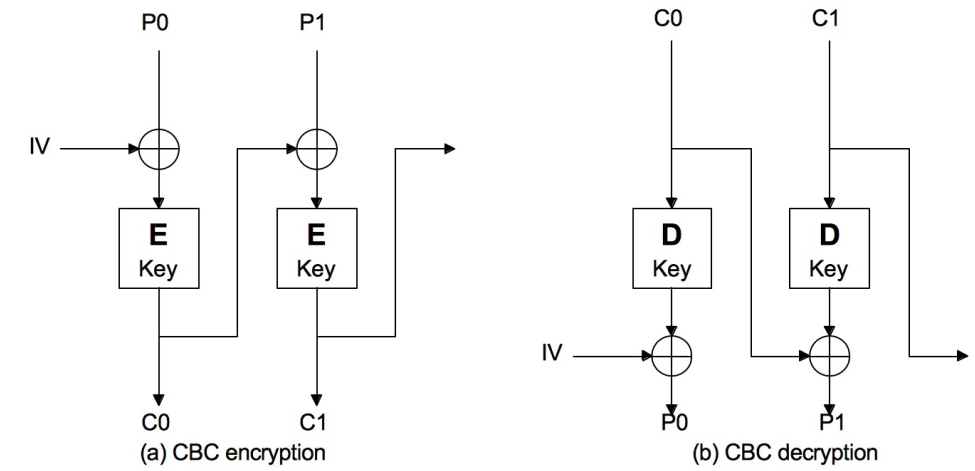
\includegraphics[width=0.3\textwidth]{Figures/TPM/CBC.png}
\end{figure}

\item \begin{lstlisting}[style=bash]
openssl enc -aes-256-cbc -e -in t.txt -out t.enc #encrypt
\end{lstlisting}
\item \begin{lstlisting}[style=bash]
openssl enc -aes-256-cbc -d -in t.enc -out t.txt #decrypt
\end{lstlisting}
\end{itemize}

\subsubsection{asymétrique}
\begin{itemize}
\item Deux clés (publique et privée) clé publique disponible par des certificats (CMD pgp)
\item Encrypt public - Decrypt private = confidentialité
\item Encrypt private- Decrypt public = signature digitale
\end{itemize}

\subsubsection{hash}

Transforme un texte, document en un nombre de N bits unique (SHA-2, SHA-3, Blake2).

\verb!md5sum file => a6a0e8d0522...! 
où
\verb!openssl dgst -md5 file!  

\subsubsection{signature}

En deux parties: 1. Calcul du HASH puis encryptage avec clé privée. 
\begin{figure}[H]
    \centering
    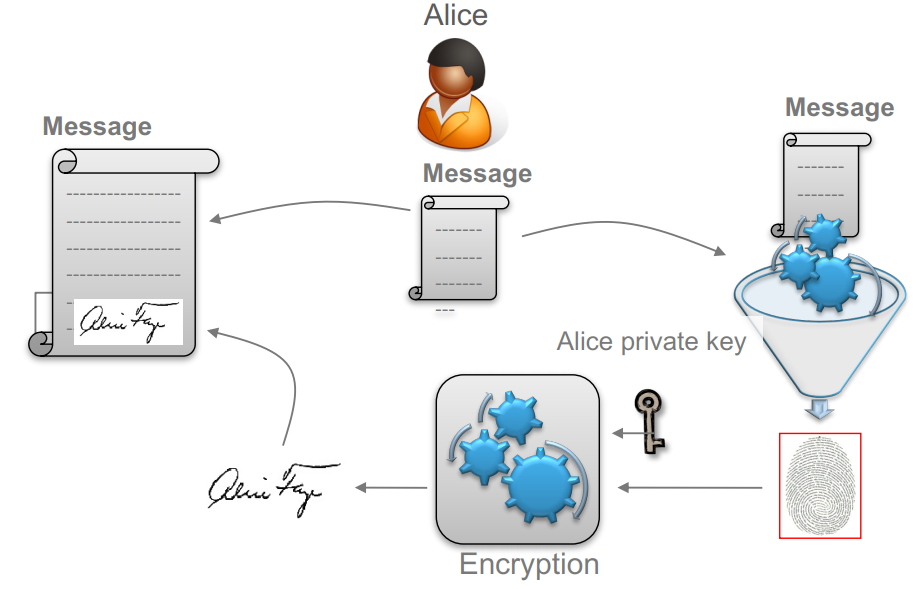
\includegraphics[width=0.3\textwidth]{Figures/TPM/signature.png}
\end{figure}

\subsection{Implémentations TPM}
\begin{itemize}
\item discrete : Circuit dédié 
\item integrated : Partie du $\mu C$ qui gère le TPM
\item Hypervisor : virtuel fournis par personne fiable
\item Software : virtuel pour faire des test pas sécurisé
\end{itemize}

\subsection{Architecture interne}

\begin{figure}[H]
    \centering
    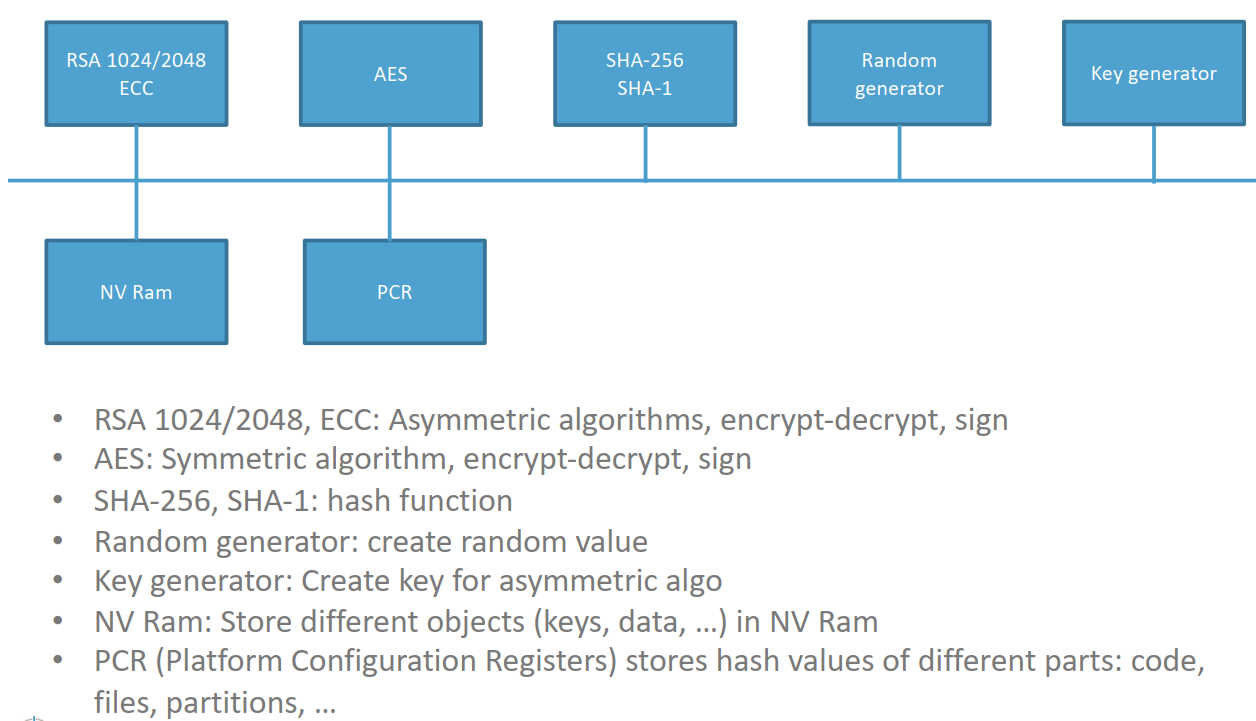
\includegraphics[width=0.3\textwidth]{Figures/TPM/internal.png}
\end{figure}

\subsection{Hiérarchies}
\begin{itemize}
\item endorsement : réservé au fabricant du TPM et fixé lors de la fabrication.
\item platform : réservé au fabricant de l'hôte et peut être modifier par l'équipementier.
\item owner : hiérarchie dédiée à l'utilisateur primaire du TPM peut être modifié en tout temps.
\item null : réservé aux clés temporaires (RAM s'efface à chaque redémarrage)
\end{itemize}

\subsection{Créer, utiliser clés}

\begin{figure}[H]
    \centering
    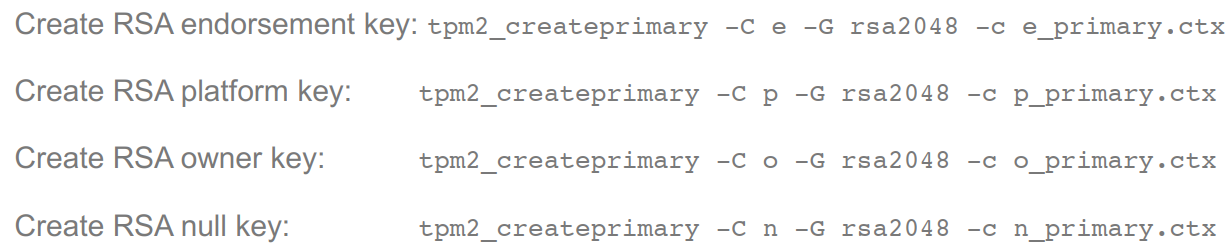
\includegraphics[width=0.3\textwidth]{Figures/TPM/createKey.png}
\end{figure}

\subsection{Commandes principales}
\begin{lstlisting}[style=bash]

tpm2_createprimary -C o -G rsa2048 -c o_prim #créer un clé primaire owner
tpm2_getcap handles-transient #voir clé dans la RAM
tpm2_getcap handles-persistent #voir clé dans la NV-RAM
tpm2_evictcontrol -c o_primary.ctx # sauver une clé en NV-RAM
tpm2_flushcontext! -t ##effacer toute la RAM
tpm2_create -C o_prim -G rsa2048 -u child_pub -r child_priv #créer clé enfant
tpm2_load -C o_prim -u child_pub -r child_priv -c child #charger clé enfant
shred passwd, rm -f passwd #supprimer de l'hôte

\end{lstlisting}

\subsection{encrypter-décrypter, signer-vérifier}
\begin{lstlisting}[style=bash]

tpm2_rsaencrypt -c child -s rsaes clearfile -o encryptedfile
tpm2_rsadecrypt -c child -s rsaes encryptedfile -o clearfile
tpm2_sign -c child -g sha256 -o file.sign file
tpm2_verifysignature -c child -g sha256 -s file.sign -m file
\end{lstlisting}

\subsection{Registres PCR}

\begin{lstlisting}[style=bash]
tpm2_pcrreset 0
tpm2_pcrextend 0:sha1=8c83...(hash)
\end{lstlisting}

\subsection{Sauver des données sur le TPM}

\begin{lstlisting}[style=bash]
tpm2_evictcontrol -c passwd.ctx 0x81010000 -C o  #sauver
tpm2_unseal -c 0x81010000 > passwd  #récuperer
\end{lstlisting}

\subsection{Sauver des données et protéger avec PCR policy}
\begin{lstlisting}[style=bash]
sha1sum passwd #calcul hash
tpm2_pcrreset 0 #flush PCR0
tpm2_pcrextend 0:sha1=8c839... #sauve hash
tpm2_createprimary -C o -G rsa2048 -c primary
tpm2_startauthsession -S session
tpm2_policypcr -S session -l sha1:0 -L pcr0_policy #créer politique
tpm2_flushcontext session

tpm2_create -C primary -g sha256 \
-u passwd_pcr0.pub -r passwd_pcr0.priv \
-i passwd -L pcr0_policy

tpm2_evictcontrol -c passwd_pcr0 0x81010000 -C o
tpm2_flushcontext session

shred passwd
rm -f passwd

tpm2_startauthsession --policy-session -S session
tpm2_policypcr -S session -l sha1:0
tpm2_unseal -p session:session -c 0x81010000 > passwd
\end{lstlisting}

\end{document}